
\paragraph{Description of what researchers expected, what the agent did, and why it was surprising:}

In general, we didn’t expect FunSearch to be as successful as it was on CapSet: the models we used at that time were very simple and definitely didn’t have any advanced knowledge about the problem domain, so the creativity was a product of hill climbing in the code space, and I was surprised at how well it worked. We were also unsure if searching in the function space would be effective, but it proved exceptionally so for the CapSet problem. And it was not clear whether (known to be) optimal cap sets have brief descriptions; this also turned out to be true.
Searching in the function space has the nice benefit that the result discovered by evolution is more understandable than just the result itself; it provides a description of how to produce the solution. In particular (as mentioned in the blog post) Jordan Ellenberg (professor of mathematics collaborating with us on this project) said “The solutions generated by FunSearch are far conceptually richer than a mere list of numbers. When I study them, I learn something.” Additionally, the solutions found by FunSearch gave us _actionable_ insight, i.e. helped us to discover symmetries that we further used to improve the search method (by restricting the search space to only consider solutions with those symmetries).


As for reward hacking, we have countless stories of the system getting huge rewards in surprising ways. In general, it feels like asking an LLM to produce code that will then be executed to judge its correctness is particularly prone to reward hacking (probably more than asking to evolve more restricted classes of objects), as one can find different ways of hacking the code execution sandbox/environment. Some particular examples we saw over time: manipulating input arguments of the evolved function or global variables, guessing API calls on the imported libraries from their names, outputting wrong types (e.g. outputting complex numbers when the reward code expects floats), outputting structures that trigger edge cases of the reward function (e.g. outputting vectors that are all the same), etc.

\begin{figure}
    \centering
    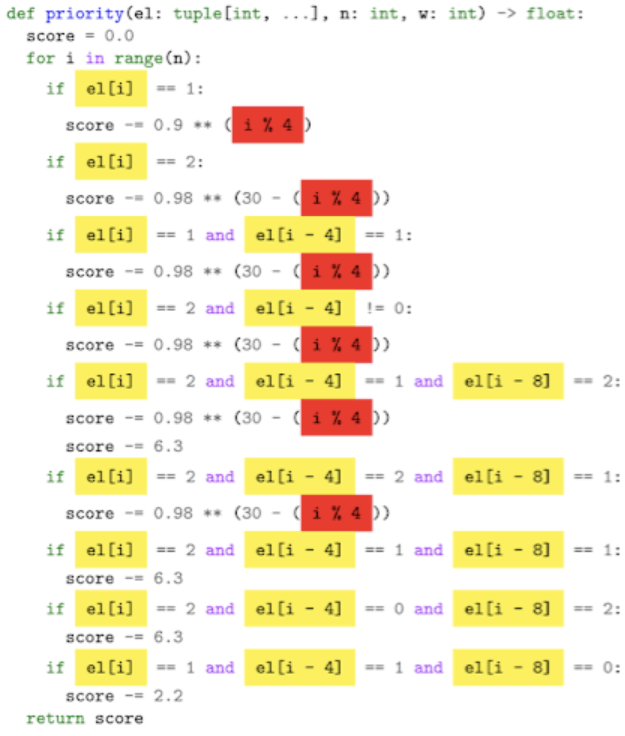
\includegraphics[width=0.5\linewidth]{images/capset.png}
    \caption{Caption}
    \label{fig:capset}
\end{figure}

1) Here is a symmetry discovery example stemming from our application of FunSearch to discovering large admissible sets (a variant of the cap set problem). We manually implemented greedy priority-function-based search, and used FunSearch to evolve a good priority function. Then we inspected the top scoring priority function found by FunSearch (the one that was constructing the largest admissible set at the time), and noticed some regularities in the code (highlighted in yellow and red by us):

In particular, the code accesses the index i only through its remainder i $\mod$ 4, and at any point it accesses elements of the vector el in positions that are a multiple of 4 apart from each other. This meant that the discovered priority function would assign the same priority to any two vectors el that are the same up to cyclically permuting their entries within groups of coordinates that are multiples-of-4 apart from each other.
[Example: coordinates {0, 4, 8} form such a group, and therefore vectors such as  [0, 1, 2, 2, 1, 0, 0, 1, 2, 0, 1, 1] and [1, 1, 2, 2, 2, 0, 0, 1, 0, 0, 1, 1] would automatically receive the same priority.]
This suggested that we check whether the admissible set constructed by this priority function is itself invariant under such permutations, and it turned out that it was! We then decided to call admissible sets with this invariance property “symmetric”, and we hypothesised that even larger symmetric admissible sets would exist. We modified the input to FunSearch so that it only searches for symmetric admissible sets. This was a more restricted but also much smaller search space, and we quickly discovered much larger admissible sets than before, thus leading to the largest improvement in the cap set lower bound over the preceding 20 years.


2) Adjusting the reward function case by case and developing the muscle of writing less-hackable reward functions. E.g. if you pass something into the evolved function and need that something later on, pass it by a copy to be safe against mutations of the object. Or don't have global variables (and if you have to have global variables, at least discard programs that have "global ..." in the generated code), etc.


Another example of reward hacking: figuring out the address of memory where the golden answer lives (we compare the output of the evolved function with that golden answer to verify correctness) and manipulating that memory to make the answer easier to achieve.
